\documentclass[a4paper]{article}
\usepackage[T1]{fontenc}
\usepackage[utf8]{inputenc}
\usepackage{lmodern}
\usepackage{amsmath,amssymb}
\usepackage[top=3cm,bottom=2cm,left=2cm,right=2cm]{geometry}
\usepackage{fancyhdr}
\usepackage{esvect}
\usepackage{xcolor}
\usepackage{tikz}\usetikzlibrary{calc}

\parskip 1.5em\parindent 0pt

\begin{document}

\pagestyle{fancy}
\fancyhf{}
\setlength{\headheight}{15pt}
\fancyhead[L]{Electromagnétisme}\fancyhead[R]{Question 49}

% Énoncé
\begin{center}
	\large{\boldmath{\textbf{RMN}}}
\end{center}

% Correction

Soit $\mathcal{R}_g$ un référentiel galiléen. Soit un proton immobile dans ce référentiel plongé dans un champ magnétique uniforme $\vv{B}$\\
$\vv{F}=e\vv{v}\wedge\vv{B}+(\vv{\mathcal{M}}\cdot\vv{\nabla})\vv{B}=\vv{0}$ car $\vv{v}=\vv{0}$ et $\vv{B}$ uniforme\\
Ainsi, un proton immobile reste immobile.\par
TMC : $\dfrac{\mathrm{d}\sigma}{\mathrm{d}t}=\vv{\mathcal{M}}\wedge\vv B$ donc $\dfrac{\mathrm{d}\vv{\mathcal{M}}}{\mathrm{d}t}=k\vv{\mathcal{M}}\wedge\vv B$. Donc $\dfrac{\mathrm{d}\vv{\mathcal{M}}}{\mathrm{d}t}\cdot\vv{\mathcal{M}}=0$ donc $\dfrac{1}{2}\vv{\mathcal{M}}^2=$ cste donc $\Vert\vv{\mathcal{M}}\Vert=$ cste.\\
De plus, $\dfrac{\partial\vv{\mathcal{M}}}{\partial t}\cdot\vv B=0$ donc $\dfrac{\mathrm{d}\vv{\mathcal{M}}\cdot\vv B}{\mathrm{d}t}=0$. Comme $\Vert\vv{\mathcal{M}}\Vert$ et $\Vert\vv B\Vert$ sont constants, $\theta=(\vv{\mathcal{M}},\vv B)=$ cste\\
$\left.\dfrac{\mathrm{d}\vv{\mathcal{M}}}{\mathrm{d}t}\right|_{\mathcal{R}_g}=\vv{\omega}\wedge\vv{\mathcal{M}}$ avec $\vv{\omega}=-\omega\vv{z}=-k_pB\vv{z}$\\
Ainsi, $\left\{\begin{array}{l} \dot x=-\omega y \\ \dot y=\omega x \\ \dot z=0 \end{array}\right.$ donc $z=$ cste et pour $u=x+iy$, on a $\dot u=-i\omega u$. Donc $u=Ae^{i\omega t}$ donc $x=A\cos\omega t$ et $y=A\sin\omega t$.\\
On a $\Vert\vv{\mathcal{M}}\Vert=\sqrt{\mathcal{M}^2\cos^2\theta+A^2\cos^2\omega t+A^2\sin^2\omega t}=\sqrt{\mathcal{M}^2\cos^2\theta+A^2}$ donc $A=\pm \mathcal{M}\sin\theta$ (on prend +)\\
Finalement, $\vv{\mathcal{M}}$ est en precession uniforme autour de $\vv z$ à la vitesse angulaire $-\omega=-k_pB$
\par

On branche un champ magnétique tournant $\vv*{B}{T}$ de vitesse angulaire $\vv{\Omega}\parallel\vv{z}$\\
TMC dans $\mathcal{R}_g$ : $\left.\dfrac{\mathrm{d}\vv{\sigma}}{\mathrm{d}}\right|_{\mathcal{R}_g}=\vv{\mathcal{M}}\wedge(\vv{B}+\vv*{B}{T})$\\
Soit $\mathcal{R}$ un référentiel tournant $\vv{\Omega}$ par rapport $\mathcal{r}_g$\\
Alors, $\left.\dfrac{\mathrm{d}\vv{\mathcal{M}}}{\mathcal{d}t}\right|_{\mathcal{R}}=-\vv{\Omega}\wedge\vv{\mathcal{M}}+k_p\vv{\mathcal{M}}\wedge(\vv{B}+\vv*{B}{T})=\vv{\mathcal{M}}\wedge(\vv{\Omega}+k_p(\vv{B}+\vv*{B}{T}))$\\
$\vv{P}=\vv{\Omega}+k_p(\vv{B}+\vv*{B}{T})$ est fixe dans $\mathcal{R}$\par
On est donc ramené à la première étude : $\vv{\mathcal{M}}$ précesse à la vitesse angulaire $P$ autour de $\vv{P}=(\Omega+\omega)\vv{z}+k_p\vv*{B}{T}$ avec $P=\sqrt{(\Omega+\omega)^2+(k_pB_T)^2}$\par
\fcolorbox{red}{white}{\textbf{Double précession :} $\vv{P}$ précesse autour de $\vv{z}$ à $\Omega$ et $\vv{\mathcal{M}}$ précesse autour de $\vv{P}$ à $P$}
\par

On suppose que $\vv{\mathcal{M}}=\mathcal{M}\vv{z}$ à $t=0$\\
On a $\vv{\mathcal{M}}\cdot\vv{P}=$ cste car $\dfrac{\mathrm{d}\vv{\mathcal{M}}}{\mathrm{d}t}=-\vv{P}\wedge\vv{\mathcal{M}}$. Donc $\alpha=(\vv{\mathcal{M}},\vv{P})=$ cste\\
A $t=0$, $\mathcal{M}(\Omega+\omega)=\mathcal{M}\vv{z}\cdot((\Omega+\omega)\vv{z}+k_p\vv*{B}{T})=\vv {\mathcal{M}}\cdot\vv P=\mathcal{M} \sqrt{(\Omega+\omega)^2+(k_pB_T)^2}\cos\alpha$\\
Donc $\cos\alpha=\dfrac{\Omega+\omega}{\sqrt{(\Omega+\omega)^2+(k_pB_T)^2}}$

\begin{minipage}{0.5\linewidth}
	Pour $\alpha=\dfrac{\pi}{4}$, $\Omega=-\omega\pm k_pB_T$ avec $\omega=-k_pB_T$\\
	Deux valeurs particulières de $\Omega$ donnent $\alpha=\dfrac{\pi}{4}$\\
	Alors, à $t=\dfrac{T}{2}=\dfrac{\pi}{\sqrt{(\Omega+\omega)^2+(k_pB_T)^2}}$, $\vv{\mathcal{M}}$ est couché
\end{minipage}
\begin{minipage}{0.5\linewidth}
  \centering
  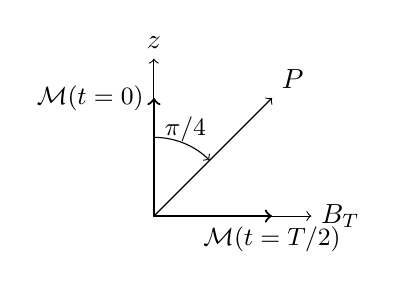
\begin{tikzpicture}
    \draw[<->] (2,0) node[right]{$\vv B_T$} -- (0,0) -- (0,2) node[above]{$\vv z$};
    \draw[->] (0,0) -- (1.5,1.5) node[above right]{$\vv P$};
    \draw[thick,->] (0,0) -- (0,1.5) node[left]{{\small $\vv \mathcal{M}(t=0)$}};
    \draw[thick,->] (0,0) -- (1.5,0) node[below]{{\small $\vv \mathcal{M}(t=T/2)$}};
    \draw[->] (0,1) arc (90:45:1);
    \node at (.4,1.1) {{\small $\pi/4$}};
  \end{tikzpicture}
\end{minipage}\par

Conclusion pratique : on peut coucher les aimants en faisant agir pendant $\frac{T}{2}$ un champ magnétique tournant convenable.\\
On pourrait aussi transformer $\vv{\mathcal{M}}(t=0)$ en $-\vv{\mathcal{M}}(t=0)$, il suffit de prendre $\alpha=\dfrac{\pi}{2}$ ie $\Omega=-\omega$


\end{document}
